%% The first command in your LaTeX source must be the \documentclass command.
%%
%% Options:
%% twocolumn : Two column layout.
%% hf: enable header and footer.
\documentclass[
% twocolumn,
% hf,
]{aiitart}
\usepackage{doi}
\def\doitext{DOI:}
\usepackage{indentfirst}

% AIIT'2022 Zrenjanin, TZFR

%%
%% One can fix some overfulls
\sloppy

%%
%% Minted listings support
%% Need pygment <http://pygments.org/> <http://pypi.python.org/pypi/Pygments>
\usepackage{minted}
%% auto break lines
% \lstset{breaklines=true}

%%
%% end of the preamble, start of the body of the document source.
\newcommand{\email}[1]{\texttt{#1}}
\graphicspath{{pics/}}
\providecommand{\LuaLaTeX}{Lua\LaTeX}

\begin{document}

%%
%% Rights management information.
%% CC-BY is default license.
%\copyrightyear{2022}
% \copyrightclause{Copyright for this paper by its authors.  Use permitted under Creative Commons License Attribution 4.0  International (CC BY 4.0).}

%%
%% This command is for the conference information
\conference{AIIT'2022
14 October, 2022, Zrenjanin, Serbia}

%%
%% The "title" command
\title{Knowledge graph based distributed infrastructure for processing documents used for organizing education process}
% Менять можно все, и заголовок.... мы тут сами по себе

%%
%% The "author" command and its associated commands are used to define
%% the authors and their affiliations.
\author[1,2]{Evgeny A. Cherkashin}
\author[2]{Victoria A. Popova}
% \cormark[1]
% \fnmark[1]
\address[1]{Matrosov Institute for System Dynamics and Control Theory SB RAS, Irkutsk, Russia}
\address[2]{Institute of Mathematics and Information Technologies, Irkutsk State University, Irkutsk, Russia\\[0.7em]
\email{eugeneai@icc.ru};\quad\email{victorypopova1@gmail.com}}

%% Footnotes
% \cortext[1]{Corresponding author.}
%\fntext[1]{These authors contributed equally.}

%%
%% The abstract is a short summary of the work to be presented in the
%% article.
\begin{abstract}
  This paper deals with the application of early developed infrastructural components based on knowledge graph data representation and knowledge-based data processing to university course documents processing, authoring and providing with their data a future platform for organization of the educational process.  Main goal of the activity is to integrate static university facade data represented as educational program documentation with university infrastructure, \emph{e.g.}, library, schedule, various existing process planning systems already made by master students and faculty.
\end{abstract}

%%
%% Keywords. The author(s) should pick words that accurately describe
%% the work being presented. Separate the keywords with commas.
\begin{keywords}
  knowledge graph \sep
  logical inference \sep
  education process automation \sep
  distributed data processing \sep
  document authoring automation
\end{keywords}

%%
%% This command processes the author and affiliation and title
%% information and builds the first part of the formatted document.
\maketitle
%     July 2020

% DOI:10.47350/ICCS-DE.2020.24
%    Proceedings of The International Workshop on Information, Computation, and Control Systems for Distributed Environments

\section{Introduction}

University is a complex sociotechnical system (STS) \cite{zh2020} comprising various components, which functioning is provided mostly by university staff and automation software.  Irkutsk state university (ISU) has quite normal (required) level of automation in the areas of accounting, education process planning, learning management, student state control, library data access.  The automation has an island character in domain and structural sense.  Institutes of ISU develop own software to solve their actual problems and do not share results between ISU community. It seems that there is no such tradition.  Some solutions are implemented by a special department of Institute of Mathematics and Information Technologies (IMIT) on request.  For example, during COVID-19 pandemics, IMIT supported Big Blue Button functioning for all departments of ISU, implemented Moodle modules for remote enrollment management.

% Неправильные термимны
% syllabus - sillabi (pl.) = Рабочая прграмма дисциплины.
% Syllabus: A list of topics or books that are planned to be studied in a particular subject.
% curriculum - curricula (pl.) = учебный план.
% Curriculum: The subjects that are included in a course of study in a college or university. (noun)
% faculty - профессорско-преподавательский состав (ППС)
% Faculty: A group of departments in a college or university that focuses on an area of study or several related subjects. (noun)
% appraisal fund - ФОС

To obey constantly rising requirements imposed on the university functioning, some areas are still experiencing a lack of automation. One of the challenging problem is course documentation preparation, such as course description mediation with an academic plan (syllabus).  In a course description (CD), in the case of contracting or changing the numbers of units (hours) spent to lecture and laboratory works, teacher must reschedule the amounts by adding/removing topics or contracting/extending a topic content.  The format of printing layout of the syllabi is altered every two years in Russia, and even unchanged content must be reconstructed.  Yet another task is to check the capabilities of the university library to supply printing editions for references of the CD, renew URL references to the electronic ones.  Another problem deals with educational process management.  There is no general system of class schedule planning and browsing, monitoring student progress, namely, the fact of attending a class and the obtained grades.  % Some departments have their localized solutions, which cannot be efficiently adapted.
% Другой проблемой, которую требуется решить непосредственно по части организации учебного процесса, является отсутствие единой информационной системы, которая бы позволила просматривать расписание занятий, а также контролировать успеваемость студентов за счёт выставления оценок и отметок о посещаемости занятий. Важно отметить, что некоторыми учебными подразделениями такие проблемы уже решены. Но разработанные информационные системы адаптированы под характеристики конкретного учебного подразделения, что не позволяет использовать ту же систему в другом подразделении. Поэтому требуются такие программные продукты, которые могли бы использовать все институты и факультеты ИГУ для решения проблем организации учебного процесса.

The abovementioned problems are solved by faculty manually using office automation software (Microsoft and LibreOffice), institute management staff develop recommendations and template documents to simplify and inspire faculty to proceed with authoring of the CDs in time and result in a good quality documents (in all aspects).  The devised manually, class schedules are published on ISU site as soon as they formed.  % In such circumstances, its reconstruction becomes inoperative.   %  Что касается задач представления расписания и контроля успеваемости студентов, такие задачи также часто решаются вручную при помощи продуктов Microsoft и LibreOffice, из-за чего  редактирование расписания занятий является неоперативным процессом, поскольку изменения будут отображаться студентам и преподавателям только после публикации документа на веб-сайте или на стенде института. При достаточном количестве человеческих ресурсов такого вида работы могут быть выполнены оперативно с низкой вероятностью возникновения ошибок.
The human factor is exposed in a degradation of the quality of requirements compliance.  This is, partially, due to the present underestimation of the role of a teacher and economic reasons: teachers often have positions in other institutions and mentally not interesting in placing this activity to the first place in their everyday schedule.

It seems that the problems can be solved by using artificial intelligence at a good level.  ISU site includes units for supplying students and faculty with the educational process documents, including curricula and CDs for the past few years for all study programs.  Documents are represented in PDF format and can be informative sources of meaningful data, as well as various documents from Russian government sites containing references books for specialties, job requirements, {\em etc}.

Other two abovementioned problems of class scheduling and student progress monitoring have many aspects of consideration, including use of combinatorial optimization engines for solving constraint satisfaction problem of scheduling, data representation for students' grades (formal and instructive), their meaningful description, compliance to educational trajectories, competence set, creative solutions, and formal tests.

% Это слишко детально для введения. Но дает мне понимание проблематики. Я не выкидываю твой труд, просто резюмирую.
%Проблемы автоматизации представления расписания и контроля успеваемости также являются решаемыми задачами, хоть и далеко не простыми. На текущий момент во многих учебных подразделениях ИГУ расписание предоставляется только в файле Word или Excel. В таких файлах расписание занятий сортируется по студенческим группам, что влечёт трудности поиска занятий преподавателем. Расписание такого формата также неудобно просматривать с мобильных устройств. Стоит отметить, что во всех учебных подразделениях ИГУ расписание отличается своим представлением, поэтому при разработке системы требуется учитывать настраивающийся интерфейс, чтобы студенты и преподаватели не испытывали трудностей при просмотре расписания  и быстро привыкли к использованию приложений для расписания.

% aaa,aaaa and other ....

% Для контроля успеваемости студентов также требуется система, которая бы позволяла добавлять оценки как в течение учебного семестра за занятия, так и предназначалась для ввода данных об зачётах, экзаменах, курсовых работах и практиках. Немаловажно учитывать и посещаемость занятий студентами. Чаще всего такие данные заполняются преподавателем на обычном бумажном листе, информация с которого может далее быть перенесена вручную на электронные устройства для, например, расчёта в программе Excel оценки или суммы баллов за учебный семестр.

The aim of the present research presented in the paper is to automate these creative activities of the faculty authoring CD, organizing processes, monitoring and control students' progress, and in the future, form a basis of educational process modelling to support the compliance checking, individual education trajectories of students.

\section{Used development platform}

The basis of our distributed warehousing is being driven by present semantic data servers, knowledge graphs (KGs) \cite{kg}, such as Virtouso \cite{virtuoso}, ClioPatria \cite{b8}, and by adapting rational databases to Semantic Web (SW) technologies~\cite{tbl} (Figure~\ref{fig:arch}).  The usage of the distributed KGs allows us developing subsystems independently, having in mind their facilities of coupling distributed data and services within common domains in a distributed network.  Using KG as data structures enables a developer to create software complexes as interacting agents via KGs' content, reaching loose coupling between them.  Another advantage of SW and KG usage is nowadays domain standardized descriptions represented as well-known vocabularies.

\begin{figure}
\centering
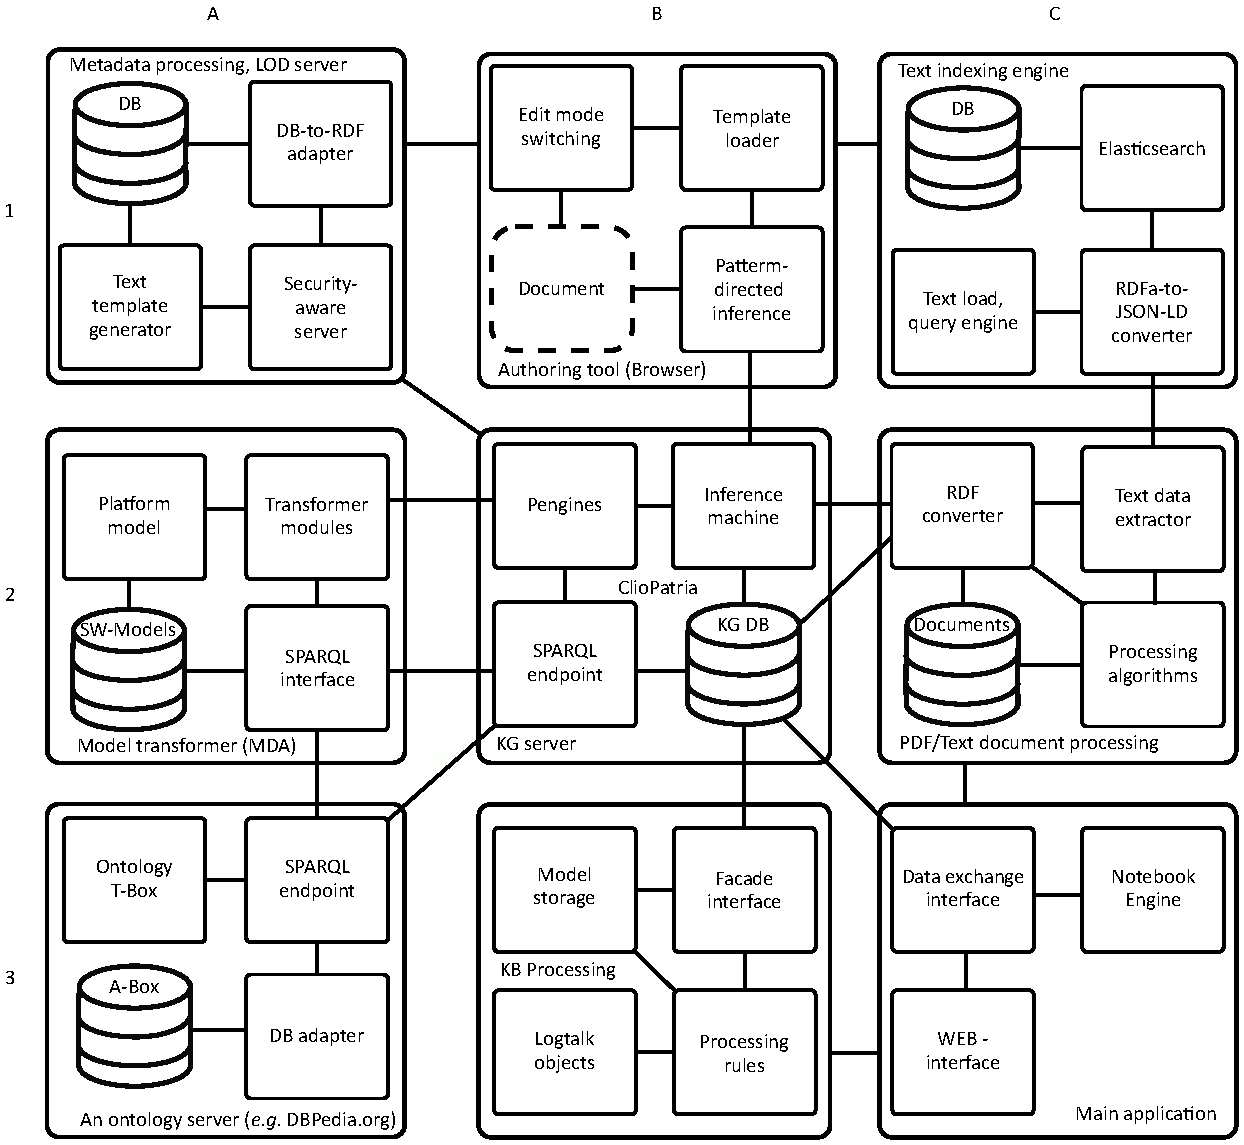
\includegraphics[width=1\linewidth]{architecture-mda-lod-ext-general.pdf}
\caption{General architecture of used KG-based software development platform}
\label{fig:arch}
\end{figure}

% Текст надо адаптировать к заджачам.
The kernel module of applications is KG server (B2) built on the base of Virtuoso with web-server and Pengines plug-ins~\cite{pengines}.  %ClioPatria is a web-application implemented in SWI-Prolog \cite{swi} being ISO-compliant Prolog implementation.  KG functions are implemented with SW package, supplied in standard SWI-Prolog distribution.
Virtuoso, as compared to ClioPatria, supports \verb|UPDATE| and \verb|DELETE| \verb|SPARQL| queries, can be scaled in a network.  Pengines service enables SW web-applications to utilize logical inference on the server-side with browser JavaScript environment integration.  Pengine's knowledge base is extended with the programmer's Prolog modules~\cite{b10,swi}.  The kernel module stores a common global part of A-~and T-boxes of applications, \emph{i.e.}, it is an application database.  Other modules provide an application (C3) that use other platform assets.

Authoring tool (B1) \cite{authoring,zont19} is used to provide document generation, and integration.  This tool allows one to implement SW document content generation utilizing templates and data from other web pages and websites providing LOD\footnote{Abbreviation of Linked Open Data} \cite{b1,c6} capabilities. The composed page can be stored in a KG as a set of triples and indexed in the text indexing module (C1).

Text indexing engine (C1) provides a service for storing documents represented as KG triples, JSONs, and BLOBS of any format with corresponding text layers.  This module has two implementations.  One is built on the Sphinx Search engine, and the second is Elasticsearch~\cite{b13}.  Elasticsearch supports JSON as the only document format and is easily integrated with KG using \verb|JSON-LD| for triple representation.  Sphinx Search is much faster in text and database records indexing and consumes less RAM as it is implemented in C++. The choice of an engine depends on the primary document representation used in the application.

BLOB stored as KGs documents having no markup (PDFs, scanned documents) usually contain valuable data to be revealed for application use.  The documents could be report data or scientific paper content, DJVU files, or raster images.  Data recognition is implemented in the PDF/text document processing module (C2), where data processing workers query the text indexing module for BLOB documents and add recognized text and high-order structure layers.  All obtained layers are stored in the database of C1, and data of general interest are to be converted in triples of KG.

A generalized KG processing is being executed in the KB processing module (B3).  This component denotes a set of rules used to implement the validating, emergent semantics derivation, and analysis and synthesis of the new data, including resultant output.  Module A2 is the source of model data (design of domains, UML, problem statement, \emph{etc.}), which is converted and form the T-boxes of a KG.  The conversion is a kind of Model-driven architecture (MDA) implementation \cite{b2}.  Transformation is carried out under the control of the platform model, describing a context of the conversion.  For example, in the case of software source code synthesis, the software platform model is used to implement model objects.

The metadata processing module (A1) denotes the environment capabilities for expressing the semantics out of the data processing modules' output and the input data semantics.  It allows us to store resultant data in KG for further usage in module (B3) for problem-solving and decision-making.  Module A3 denotes external services and KG with valuable resources, \emph{e.g.}, DBPedia~\cite{b3} global objects.

\section{Processing course description documents}

As it was told above, the input consist of PDF documents of CD downloaded from the website of ISU.  The document should first be analyzed to obtain meaningful data, which can be processed imperatively.  It is usually possible as the PDFs are generated from MS Word documents (not scanned).  For a CD, meaningful information is the title and the code of the course, list of topics, distribution of study units (academic hours) between lectures, practice, seminars, personal work of student, list of questions for knowledge assessment, \emph{etc}.

The PDF processing is carried out by converting source PDF to XML by \verb|Poppler| library.  The XML file is processed by authors' set of utilities implemented as knowledge-based systems in Logtalk \cite{logtalk} object-oriented (OO) logical programming language.  Preliminary input data conversion represents XML tree (list of pages with lists of runs, lines and font definitions) into an in-object database, each element is numbered to conserve orders, neighborhood elements of the similar quality are marked to organize fast access to successor elements.

The system recognizes basic features of each run (a sequence of characters having a common style) and line, \emph{e.g.}, is it a hanging line of a paragraph, or does it have a number at the start of its text.  For all text lines of a page, we figure out the bounding box, excluding page numbers (one or two character strings at upper or lower edge of page with number that equal to the PDF page number). These features are used to join runs and rows into paragraphs, the bounding box is also used to figure out regular paragraph lines.  Each join is accompanied of figuring out paragraph geometry. Paragraphs, which were separated by page breaks, are reconstructed at the second stage, using additional rules.

The next stage is CD structure recognition.  Each institute of ISU has templates for CD authoring, so that the sequences and styles of the headers are similar but varying between institutions.  The headers are recognized by their numbers in a template, verifying a sequence of roots of comprising words.  The template variations are accounted by specifying a \verb|categories| of special rules, adjusting parameters of general rules and adding special ones.  Then all lines/paragraphs are associated to the header preceding them.  The headers and subheaders are in hierarchical relations too.  So, at this stage, we have a tree of basic document structures.

After constructing the hierarchy, the process of list recognition is launched.  We suppose that bullet lists have a deeper level of folding as compared to numbered ones.  The process has two stages: running through all list-like structures and find common sequences of constantly increasing numbers or same bullet symbols trying to conserve possible folding, and folding itself.  If a one-line list is found, this case is considered as a false positive list item, and it is joined to the previous paragraph as a regular line.  This rule recognizes, \emph{e.g.}, page numbers in references.  At this stage of R\&D we ignore description lists which lines start from a noun that follows a colon and other text.

The last stage is meaningful content acquisition.  At this stage, the data about header contexts and list folding are significant, they constrained the set of paragraphs, where meaningful data are located.  A location is specified with the context and a list of preceding word roots and punctuation. The target data are extracted with regular expressions or other string processing procedures.

The main OO programming technique used in implementation of PDF documents analysis is object extension and composition.  The XML-data of a document is encapsulated as a parametric Logtalk object \cite{logtalk}, which parameter is its path name.  The object provides basic input-output functions, conversion from a tree to the database, database content modification conserving consistency, debug printing, and so on.  It is extended to a recognition object (RO) by importing a set of \verb|categories| implementing analysis and synthesis stages, a set of configuration predicates are added as well.  RO is constructed aimed at a special case of syllabus template, so the imported categories are extended by descendants improving recognition capabilities.  As compared to the present component frameworks, configuration is realized with the same programming structures as a predicate implementation thanks to the abstract syntax of Prolog/Logtalk, and, moreover, configuration parameters also can be rules deducing values.  The extracted data are converted to a local KG, which added to the remote KG storing all syllabi data.

\subsection{Authoring and generating a course description}

CD data stored in a KG are filled in \LuaLaTeX{} template based on a special \LaTeX{} class \verb|sucourse|, a subclass of a KOMA-script \verb|scrartcl|, having special commands and environments for defining distributions of study units for various educational activities via keywords.  Let us consider an example of a list of laboratory works definitions expressed with the special \LaTeX{} environments.

\begin{minted}{latex}
\begin{labworks}[comp={PC-4,PC-12}] % A ``default'' competence codes satisfied by these
                                    % set of laboratory works.
. . .                               % The previous problem definitions
\begin{work}[comp={PC-4}, % a competence satisfied by this work
    hours=16,             % academic hours assigned for the task
    topics={4},           % Lecture topic for the work
    label=lw:distr]       % A LaTeX Reference \label...
    {Construction of a distributed computational system} % The title of the work
\paragraph{Problem definition:} Implement a cluster-based data processing according
to ``Map-reduce'' scheme.
\paragraph{Given} the results of the previous laboratory works.
\paragraph{Devise} a network of interconnected services realizing data flow processing.
\paragraph{Advanced level:} Organize a flow control with a RabbitMQ server.
\end{work}
\end{labworks}
\end{minted}

For example, the laboratory works are defined with two environments \verb|labworks| that setups an enumeration environment and an RDF context for SW data acquisition, and \verb|work| defining a concrete problem definition.  % Command \verb|\paragraph| is also redefined to support RDF data extraction.
The functionality of environments used is defined with so-called new \LaTeX{} extended syntax, allowing the programmer to control types of parameters.  % Here, we present an example of the environment definitions. Keyword processing are omitted as they contain too many details.
The current alpha version of class \verb|sucourse| is published at Github \cite{ghs}. % Вставь эту ссылку в список литры, я потом туда URL помещу.

\begin{minted}{latex}
\NewDocumentEnvironment{works}{O{}} % An extended synax environment definition with keywords
{ % Rexecutes at \begin{...work}
  \def\itemname{Student work} % A ``Student work'' tile placeholder
  \begin{syll@items}[#1]  % Processing keywords by a private environment
  \begin{rdfctx}{\rdfsetctx{list}{syll wpdd:itemList % Semantic web item list definition
       !wpdd:ExampleList !wpdd:CurrentAttestation !wpdd:ItemList}}
  \def\syllabus@worktype{wpdd:LaboratoryWork} % RDF type of itemsin in an extended Jinja
}                                             % equation syntax
{ % Executes at \end{...work}
  \luadirect{ syll.items:workValidation() } % Run [table] data validation
\end{rdfctx} % End of a RDF context
\end{syll@items} % End of parent environment
}

\NewDocumentEnvironment{labworks}{O{}} % Specializes ``works'' environment
{
\syl@labwork@section % Starts section with name from a template adapter
\begin{works}[totalnames={'hours'},
  type=labwork,      % A kind of time units to account (labworkd, lectures ...)
  itemname={Laboratory work},  % Set item naming ``Laboratory work N.''
  rdftype={LaboratoryWork},#1]}% Set RDF type of items.
{\end{works}}

\NewDocumentEnvironment{work}{O{}m} % Define a work with a mandatory title
{
  \begin{syll@item}[#1]{#2} % Setup item with a parent assets
  \begin{rdfenv}{list ^schema:member !wpdd:ListItem
     !wpdd:Example \luadirect{self.item:sprintRDFTypes()} }
  \paragraph{{\workheaderstyle \itemname\ \theitem.}~{\worktitlestyle #2}}
     % A format of the beginning of an item.
}
{
\end{rdfenv}\par\vspace{1em} % Add an empty line between items
\end{syll@item}
}
\end{minted}

The environments implicitly execute \verb|Lua| code for collecting data, checking constraints and generating tables and other \TeX{} structures of a syllabus.  If constraints are not satisfied, an error message is added as red color text into the \TeX{} source.   The validation can be turned off by \verb|final| option to class. (the \verb|draft| option forces check results to be included in the resulting PDF even it is correct).
Lua's code also generates auxiliary files with data that are to be processed between \verb|lualatex| tool executions.

The latter feature is used to check library capability to support printed editions, and renew URL references for electronic ones.  This service is implemented asynchronously using RabbitMQ server to organize workflows in LAN.  One of KG subgraphs stores editions' data (caching), and texts of the references are substituted.  Other collected data from \LaTeX{} markup of syllabi is sent to KG as well.

The usage of \LuaLaTeX{} as the main text processing unit is dictated by its outstanding text layout quality capabilities, high-level markup by new commands and environments, true type font availability, and Lua support as an extension language allowing one to communicate with a parallel process in a convenient way.  Special commands prevent user to change styles, also by defining useful new structures we can support development the documents with a common text structures representing various aspects of syllabus.  A typical example is tests, which can be integrated in a document and then be exported into a format understood by LMS Moodle.

Initial state of a \LuaLaTeX{} syllabus representation is generated by Python and an RDF extended Jinja templating engine.  Jinja was improved with syntax structures allowing one to query KG or its local subgraph for triple data.  There are value-like queries with \verb|rdf:type| restrictions, and environments for answer set processing and a context definition.  Results of a template rendering also include a semantic markup invisible in the terminal PDF, but allowing one to untangle RDF data from \LuaLaTeX{} syllabi sources (alike RDFa for HTML).

\section{Scheduling}

Devising of the schedule is a well-known problem.  ISU requirements to the complexity of the solution are rater soft. This is because many requests for the schedule are difficult to formalize, and they are already considered during manual editing. The schedule currently is not compiled centralized, but for each institute or faculty separately, it is necessary that the program generates a schedule at the same time for only one academic unit (institute).

To form a schedule of a good quality (satisfying faculty and students' groups as well as possible, minimizing class resources), it is necessary to take into account a number of constraints, such as a ban on free time intervals instead of classes, control of the capacity of classrooms, various requests of faculty, for example, which days are more convenient to conduct classes, the maximum number of classes per day, \emph{etc}.  Although it is not always possible to account all the requests for the schedule, the ISU requires a system that could make a preliminary version of the schedule with the possibility of a convenient manual editing.

To devise a schedule, the constraints must be presented in a structured format that the system is capable to load and process.  To form the constraints' set directing the scheduling, it is necessary to use the following source data:
\begin{itemize}
    \item for classroom: the number of seats, the availability of a projector, computers, \emph{etc}.;
    \item for faculty (preference and requests):
    \begin{itemize}
        \item number of working days per week;
        \item maximum number of classes per day;
        \item the desired schedule of classes during the school week (compact, evenly, no preference);
    \end{itemize}
    \item for student groups:
    \begin{itemize}
        \item academic load (the total number of academic hours in each discipline, as well as the number of classes per week);
        \item number of students in groups;
        \item features of classes (streams, electives, \emph{etc});
        \item last name, first name and patronymic of the teacher for each pair;
        \item desired classroom for specific course class.
    \end{itemize}
\end{itemize}

Presently, the ISU schedule is compiled separately by each unit.  ISU institutes make a schedule using Excel spreadsheets, or do it completely manually on a sheet of paper. The software is also used in the scheduling process in some institutes. For example, at the IMIT of ISU, the program ``AUTO Schedule'' is used for scheduling, which allows a user to work with schedules of various degrees of complexity. The program can take into account the constraints listed above.

The program ``AUTO Schedule'' makes it possible to facilitate and automate the complex work of the schedule compilers as much as possible. The system helps to build, adjust easily and print the schedule in a convenient form  and visual documents. The difficulty lies in the fact that such a program does not allow integration with other university systems, that's why the user has to enter all the data about the educational process manually.  At the same time, all such data is stored in the ISU corporate information system <<1C:University>>. Therefore, the most convenient way of the integration would be an automatic downloading data about the educational process, forming the basis of a schedule compilation. Since the program ``AUTO Schedule'' has no open API, it does not allow downloading data about the educational process, the development of a system for scheduling with the possibility of the integration with the system <<1C:University>> is an actual task that could be done using the platform.

%/GA's /

The new scheduling program version must load collected data from KG.  To achieve these requirements, one is to construct a knowledge-based system inferring data from KG contents.  The main source of the data are the curricula, faculty assignments to the courses, which also must be implemented, and institute resource descriptions, which have also somewhat dynamic nature.

\section{Related implementations in other high schools}

During the search of analogues and working in collaboration with other high schools of Irkutsk and Saint-Petersburg, we collected data about their software experience, which will be projected to our requirements.

Saint-Petersburg Electrotechnical University (ETU) developed a system for study program development automation \cite{leti}. % https://etu.ru/en/university/
The system enables faculty entering the meaningful information in to a JSON-base storage by filling in forms.  Each document is represented as a JSON-structure.  CDs are generated into \LaTeX{} sources and processed into PDF.  Chair secretary obtains the PDFs and publish them a course home page.  The system is constantly developed in a department.  At present, faculty member roles and document flow is realized, \emph{e.g.}, the documents are verified by a role dealing with standard compliance.  The state of a document is presented in a user interface.  The system is capable to store arbitrary PDF documents and generate whole package of documents to present qualification authorities.

Less improved generator is developed in National Research State Technical University (NRTU) \cite{nrtu} % https://eng.istu.edu/
A server-based PHP application is loaded with curricula from well-known in Russia program ``Shakhty'', presents a user interface to define formal parts of the syllabus, such as lecture topics, list of laboratory works, personal works and seminars with the distribution of study units between them.  At the final stage, a Word document in \verb|docx| format is generated.  It should be filled in manually with other data, namely, list of tests, exams questions, literature references, \emph{etc}.

The similar principle of helping teachers is in the base of Lan' book publisher \cite{lanbook}, but their system is oriented on an automation of electronic editions collecting for a CD's syllabus.  The information system stores all the books structuring by domain tag set and delivers content to the user filtered by similar topics regarding the set of the previous chosen exemplars.

Googling the Russian part of the Internet results in more examples of syllabi generators, quick review of their user guides reveals a common direction of the development to improve generation capabilities.  In our R\&D we are to construct a system which uses the existing structured and unstructured data to construct an information model of an education process of an ISU institute and scale the results to other departments.

\section*{Conclusion}

At present stage of the research, we implemented a set of services on the base of a developed Knowledge Graph (Semantic Web) based infrastructure.  The infrastructure's modules' processing is based on active use of metadata, distributed and remote semantic resources.  It enables us to construct our solution in a multiagent fashion, where agents are independent of each other, provide a common domain for data structure devising.

Among the quite successive direction of our development are two subprojects we told about in this paper:
\begin{itemize}
    \item course description data structure recognition from PDF documents, and
    \item their generation using a new curriculum and the recognized data.
\end{itemize}
Further development will be carried on in two main directions;
\begin{itemize}
    \item improving quality of recognition with software processing tables from PDF documents using open software of our colleagues \cite{Shigarov_2016,Shigarov_2017},
    \item implementing a schedule compiling software with input data inferred from KG collected data.
\end{itemize}

% TODO: in Conclusion say about RDFa to allow user knowing nothing about LaTeX.

\begin{acknowledgments}
The results were obtained within the state assignment of the Ministry of Education and Science of Russia, the project ``Methods and technologies of a cloud-based service-oriented digital platform for collecting, storing and processing large volumes of multi-format interdisciplinary data and knowledge based on the use of artificial intelligence, a model-driven approach, and machine learning'', No.~FWEW-2021-0005 (State registration No.~121030500071-2), the network infrastructure of the Telecommunication center of collective use ``Integrated information-computational network of Irkutsk scientific-educational complex'' (\url{http://net.icc.ru}) was used as well.
\end{acknowledgments}


\begin{thebibliography}{99}
\bibitem{zh2020} Z. Stojanov, J. Stojanov, G. Jotanovic, D. Dobrilovic. Weighted networks in socio-technical systems: Concepts and challenges. CEUR-WS Proceedings of the 2nd International Workshop on Information, Computation, and Control Systems for Distributed Environments Irkutsk, Russia, July 6-7, 2020. p.~265--276.
\bibitem{kg} Hogan A., Blomqvist E., Cochez M., D’Amato C. \emph{et al}. Knowledge Graphs -- 2020 URL:\url{https://arxiv.org/abs/2003.02320v5} (access date: 12-Dec-2021)
\bibitem{virtuoso} Erling O. Virtuoso, a Hybrid RDBMS/Graph Column Store // IEEE Data Eng. Bull. 2012. Vol. 35 -- pp.~3--8.
\bibitem{b8}
  J. Wielemaker, W. Beek, M. Hildebrand, J. Ossenbruggen, ClioPatria: A
  SWI-Prolog infrastructure for the Semantic Web, Semantic Web.
  Vol. 7(5). P. 529--541 (2016) \doi{10.3233/SW-150191}
\bibitem{tbl} T.~Berners-Lee, J.~Hendler, O.~Lassila.  The semantic web: A new form of web content that is meaningful to computers will unleash a revolution of new possibilities.  Scientific American, May 2001.
\bibitem{pengines} T.~Lager, J.~Wielemaker. Pengines: Web Logic Programming Made Easy.  Theory and Practice of Logic Programming, volume~14, No.~4-5, 2014, pp.~539--552. \doi{10.1017/S1471068414000192}
\bibitem{b10}
  J. Wielemaker, G. Schreiber, B. Wielinga, Prolog-based infrastructure
  for RDF: scalability and performance, In: D. Fensel, K. Sycara,
  J. Mylopoulos (eds) The Semantic Web -- ISWC 2003. ISWC 2003. Lecture
  Notes in Computer Science. Vol. 2870. Springer, Berlin,
  Heidelberg, 2003.
\bibitem{swi} J.~Wielemaker, T.~Schrijvers, M.~Triska, T.~Lager. SWI-Prolog. Theory and Practice of Logic Programming, volume~12, No.~1-2, pp.~67--96, 2011, ISSN~1471-0684.
\bibitem{authoring} E.~Cherkashin, A.~Shigarov, V.~Paramonov, A.~Mikhailov, Digital archives supporting document content inference, Procs.  of 42-nd International Convention on Information and Communication Technology Electronics and Microelectronics (MIPRO), May 20–24, 2019.  pp. 1037-1042. \doi{10.23919/MIPRO.2019.8757196}
\bibitem{zont19} Cherkashin E., Shigarov A., Paramonov V. Representation of MDA transformation with logical objects // Procs. of International Multi-Conference on Engineering, Computer and Information Sciences (SIBIRCON) Novosibirsk, Russia -- 2019 -- pp.~0913--0918 \doi{10.1109/SIBIRCON48586.2019.8958008}
\bibitem{b1} Ch. Bizer, N. Heath, T. Berners-Lee, Linked data -- the story so
  far, International Journal on Semantic Web and Information Systems.
  2009. Vol. 5 (3). P. 1--22. \doi{10.4018/jswis.2009081901}.
\bibitem{c6} N. Heino, S. Tramp, N. Heino, S. Auer, Managing web content using linked data principles – combining semantic structure with dynamic content syndication, Computer Software and Applications Conference (COMPSAC), 2011 IEEE 35th Annual. pp. 245 - 250.  \url{http://svn.aksw.org/papers/2011/COMPSAC_lod2.eu/public.pdf}
\bibitem{b13}
  R. Kuć, M. Rogoziński, Mastering Elasticsearch - Second edition, Packet
  Publishing. 372 p. (2015)
\bibitem{b2} Cherkashin E., Terehin I., Paramonov V. New transformation approach for Model Driven Architecture // Proceedings of the 35th International Convention MIPRO, Opatija -- 2012 -- pp.~1082-1087.
\bibitem{b3}
  J. Lehmann, R. Isele, M. Jakob, A. Jentzsch, D. Kontokostas, \textit{et al},
  DBpedia -- a large-scale, multilingual knowledge base extracted from
  Wikipedia, Semantic Web Journal. Vol. 6, No. 2, P. 167--195,
  IOS Press (2015)
\bibitem{logtalk}Moura P. Programming Patterns for Logtalk Parametric Objects // In: Abreu, S., Seipel, D. (eds) Applications of Declarative Programming and Knowledge Management. INAP 2009. -- Lecture Notes in Computer Science -- Vol. 6547 -- Springer, Berlin, Heidelberg -- 2011. \doi{10.1007/978-3-642-20589-7_4}
\bibitem{ghs} A \LuaLaTeX{} class for authoring syllabi, URL:\href{https://github.com/eugeneai/sucourse} (access date: 10.10.2022)
\bibitem{leti} ETU “LETI”, URL:\url{https://etu.ru/en/university/} (access date: 10.10.2022)
\bibitem{nrtu} INRTU is a university with the best traditions\ldots, URL:\url{https://eng.istu.edu/} (access date: 10.10.2022)
\bibitem{lanbook} LMS  Lan', URL:\url{} (in Russian) (access date: 10.10.2022)
\bibitem{Shigarov_2016}
A. Shigarov, V. Paramonov, P. Belykh, A. Bondarev, Rule-based canonicalization of arbitrary tables in spreadsheets, In: G. Dregvaite, R. Damasevicius (eds) Information and Software Technologies. ICIST 2016.
\bibitem{Shigarov_2017}
A. Shigarov, A. Mikhailov, ``Rule-based spreadsheet data transformation from arbitrary to relational tables,'' Information Systems, 71, (2017). \doi{10.1016/j.is.2017.08.004}
% \bibitem{GT} Belghiat A., Bourahla M.. UML Class Diagrams to OWL Ontologies: A Graph Transformation based Approach // International Journal of Computer Applications -- Vol. 41 -- pp.~41-46.
\end{thebibliography}

\end{document}

%%
%% End of file

%%% Local Variables:
%%% mode: latex
%%% TeX-master: t
%%% End:
